\part{Ciclos de vida}

\paragraph{Ciclo de vida}  Sucesión de etapas por las que pasa el software desde que se concibe hasta que se deja de utilizar.

\paragraph{Etapa del ciclo} Lleva asociada una serie de tareas y de documentos \textit{(en sentido amplio: software)} de \textbf{salida} que serán la \textbf{entrada} de la fase siguiente.

\paragraph{Elección de un ciclo de vida} Se realiza de acuerdo con la naturaleza del proyecto, los métodos a usar, y los controles y entregas requeridos.

\section{Ciclo de vida en cascada}
\begin{figure}[H]
   \centering
   \includegraphics[width=0.7\linewidth]{Resources/cicloCascada}
   \caption{Etapas del ciclo de vida en cascada.}
   \label{fig:procesoCascada}
\end{figure}
El ciclo de vida en cascada es el más antiguo, surgido directamente de la copia del ciclo convencional de una ingeniería. Exige un enfoque sistemático y \textbf{secuencial} del desarrollo de software. Se dice que el modelo en cascada está guiado por documentos, ya que \textbf{nunca empieza la siguiente fase antes de que presente el documento de la anterior} (Tabla \ref{tab:cascadaDocumentos}).\\

\begin{table}[H]
   \centering
   \resizebox{\textwidth}{!}{%
      \begin{tabular}{|l|l|}
         \hline
         \multicolumn{1}{|c|}{\textbf{Proceso}} & \multicolumn{1}{c|}{\textbf{Documentos Producidos}}        \\ \hline
         Especificaciones del sistema.          & Especificación funcional. Arquitectura del sistema         \\ \hline
         Análisis de requisitos                 & Documento de requisitos                                    \\ \hline
         Diseño de la arquitectura del software & Especificación de la arquitectura                          \\ \hline
         Diseño de interfaces                   & Especificación del diseño                                  \\ \hline
         Codificación                           & Código de programa                                         \\ \hline
         Prueba de unidades                     & Informe de pruebas de unidad                               \\ \hline
         Prueba de módulos                      & Informe de pruebas de módulo                               \\ \hline
         Prueba de integración                  & Informe de prueba de integración y manual de usuario final \\ \hline
         Prueba del sistema                     & Informe de prueba del sistema                              \\ \hline
         Prueba de aceptación                   & Sistema final más la documentación                         \\ \hline
      \end{tabular}%
   }
   \caption{Ejemplo de documentos producidos en un ciclo de vida en cascada. \textit{No tiene que tener exactamente las mismas fases que el ciclo en cascada por defecto.}}
   \label{tab:cascadaDocumentos}
\end{table}

\subsection{Fases}
\begin{enumerate}

   \item \textbf{Ingeniería y análisis del sistema}: Define las interrelaciones del software con otros elementos del sistema más complejo en el que esté englobado; es decir, se asignan funciones del sistema al software. Por tanto, comprende los requisitos globales a nivel de sistema, mediante un análisis y diseño a alto nivel.

   \item \textbf{Análisis de requisitos del software}: Análisis detallado de los componentes del sistema implementados mediante software incluyendo \textbf{datos} a manejar, \textbf{funciones} a desarrollar, \textbf{interfaces}, y \textbf{rendimiento} esperado.
   
   \textbf{Nota:} \textit{Los requisitos, tanto del sistema como del software, deben documentarse y revisarse con el cliente.}

   \item \textbf{Diseño}: En cuanto a estructura de los datos, arquitectura de las aplicaciones, estructura interna de los programas, y las interfaces. Es un proceso que traduce los requisitos en una representación del software que permita conocer la arquitectura, funcionalidad e incluso la calidad antes de codificar.

   \item \textbf{Codificación}: Traducción del diseño a un formato que sea legible para la máquina.
   
   \textbf{Nota:} \textit{Como se puede observar, estas primeras fases del ciclo de vida consisten básicamente en una traducción de documentos.}

   \item \textbf{Prueba}: Verificar que no se hayan producido errores en alguna de las fases de traducción anteriores. Deben probarse todas las sentencias de todos los módulos, y no solo los casos ``normales''.

   \item \textbf{Utilización}: Entrega del software al cliente y comienzo de su vida útil. Es una etapa que se solapa con las posteriores.
   
   \item \textbf{Mantenimiento}: El software sufrirá cambios a lo largo de su vida útil debido a que el cliente detecte errores, que se produzcan cambios en alguno de los componentes del sistema, o que el cliente requiera modificaciones funcionales. Estos cambios requieren volver atrás en el ciclo de vida (etapas de codificación, diseño o incluso análisis), en función de la magnitud del cambio.
   
   \textbf{Nota:} \textit{El modelo en cascada, a pesar de ser lineal, contiene flujos que permiten la vuelta atrás. Además del mantenimiento, se puede volver desde cualquier fase a la anerior si se detectan fallos. Estas vueltas atrás no son controladas y quedan reflejadas en el modelo.}

  \item \textbf{Sustitución}: Cualquier aplicación acaba siendo sistituida. Es una tarea que debe planificarse cuidadosamente y, si es posible por fases:
  
  \begin{enumerate}
      \item Trasvase de la información que maneja el sistema viejo al formato del nuevo.
      \item Mantención de los dos sistemas funcionando en paralelo para comprobar que el nuevo funciona correctamente.
      \item Sustitución completa del sistema antiguo.
  \end{enumerate}
\end{enumerate}

\subsection{Aportaciones}
\begin{itemize}
   \item Es el más simple, conocido y fácil de usar.
   \item Los procesos definidos se \textbf{formalizan} en normas, \textit{sabes lo que tienes que hacer en cada momento}.
   \item Permite generar software eficientemente, y de acuerdo a las especificaciones: no sobrepasar fechas de entrega ni costes esperados.
   \item Al final de cada fase, los interesados pueden comprobar el estado del proyecto.
\end{itemize}

\subsection{Problemas}
\begin{itemize}
   \item En realidad los \textbf{proyectos no siguen un ciclo de vida estrictamente secuencial}, sino que siempre hay iteraciones. Un claro ejemplo de ello es la fase de mantenimiento, aunque es frecuente detectar errores en cualquiera de las otras fases. 
   \item No siempre se pueden establecer los requisitos desde el primer momento, sino lo normal es que se vayan aclarando y refinando a lo largo de todo el proyecto. Es habitual que los clientes no tengan el conocimiento de la importancia de la fase de análisis, o bien no hayan pensado en detalle qué quieren del software.
   \item Hasta que se llega a la fase final, no se dispone de una versión operativa del programa. Esto no resulta óptimo, dado que la mayor parte de los fallos suelen detectarse una vez el cliente puede probar el programa; al final del proyecto, es cuando más costosos son de corregir, y cuando más prisas hay.
   \item Se producen estados de bloqueo, dado que una fase no puede comenzar sin los documentos de salida de la anterior.
\end{itemize}

\textbf{Nota:} \textit{A pesar de ello, es mucho mejor desarrollar software siguiendo el modelo de ciclo de vida en cascada, que hacerlo sin ningún tipo de guías.}


\section{Construcción de prototipos}

Este ciclo de vida palia directamente las deficiencias del ciclo de vida en cascada de que:

\begin{itemize}
   \item Sea difícil tener claros todos los requisitos al inicio del proyecto.
   \item No se disponga de una versión operativa del programa hasta las fases finales.
\end{itemize}

\subsection{Sistemas que resultan ser buenos candidatos}

\begin{itemize}
   \item Resulta idóneo en \textbf{proyectos con un nivel alto de incertidumbre}, donde los requisitos no están nada claros en primera instancia, ya que se provee un \textbf{método para obtener los requisitos de forma fiable} a través del feedback del usuario. Por lo tanto, debería omitirse ante problemas bien comprendidos.
   \item También es de especial interés en aplicaciones que presenten mucha interacción con el usuario, o algoritmos evolutivos.
   \item La aplicación no debe contar con una gran complejidad, o las ventajas de la construcción de prototipos se verán superadas por el esfuerzo de un prototipo que habrá que desechar o modiificar mucho.
   \item El cliente debe estar dispuesto a probar un prototipo.
\end{itemize}

%Foto de ciclo prototipos
\begin{figure}[H]
   \centering
   \includegraphics[width=0.7\linewidth]{Resources/construccionPrototipos.png}
   \caption{Etapas del paradigma de la construcción de prototipos.}
   \label{fig:construccionPrototipos}
\end{figure}

\subsection{Beneficios de los prototipos}

\begin{itemize}
   \item Permiten probar la eficiencia en condiciones similares a las que existirán durante la Utilización del sistema.
   \item Permiten mostrar al cliente la E/S de datos en la aplicación, para detectar problemas en la especificación.
   \item Gran parte del trabajo realizado puede ser utilizado en el diseño final. El diseño se paracerá cada vez más al del producto final, meintras que los componentes codificados deberán ser generalmente optimizados.
   \item Los prototipos permiten analizar \textbf{alternativas y viabilidades}, refinando el resultado final o abortándolo antes de invertir demasiado dinero en el mismo.
\end{itemize}

\subsection{Formas de prototipos}

\begin{itemize}
   \item En papel o ejecutable, que describa la interacción con el usuario.
   \item Que implemente subconjuntos de la funcionalidad requerida, para evaluar el rendimiento.
   \item Que realice todo o en parte, pero con características que todavía deban ser mejoradas.
\end{itemize}

\subsection{Construcción de un prototipo}

\begin{enumerate}
   \item Realizar un modelo del sistema a partir de los requisitos conocidos. No es necesario realizar una definición completa de estos.
   \item Diseñar rápidamente el prototipo, centtrándose en la arquitectura del sistema y en las interfaces, antes que en aspectos procedimentales.
   \item Construir el prototipo, mediante una codificación rápiday que facilite el desarrollo incremental. Es irrelevante la calidad obtenida.
   \item Presentar el prototipo al cliente para que lo pruebe y sugiera modificaciones.
   \item Con estos comentarios, proceder a construir un nuevo prototipo, y así sucesivamente, hasta que los requisitos queden completamente formalizados y se pueda comenzar a desarrollar el producto final.
\end{enumerate}

\textbf{Nota:} \textit{Como se puede comprobar, el prototipado es una técnica que sirve fundamentalmente para la fase de análisis de requisitos.}\\

\textbf{Nota:} \textit{El prototipo no es el sistema final.}

\subsection{Problemas}
\begin{itemize}
   \item En muchas ocasiones, el prototipo, que carece de calidad, pasa a ser parte del sistema final por presiones, o bien por que los técnicos se hayan acostumbrado a él.
   \item Es \textbf{posible que nunca se llegue a la fase de construcción} por falta de recursos, lo cual da lugar a los problemas característicos de un software construido sin seguir procesos de ingeniería al emplear el prototipo como sistema final.
   \item Es imposible una \textbf{predicción de costes} fiable.
\end{itemize}


\section{Ciclo de vida incremental}
% foto de incrementos
\begin{figure}[H]
   \centering
   \includegraphics[width=0.7\linewidth]{Resources/cicloIncremental.png}
   \caption{Etapas del ciclo de vida incremental.}
   \label{fig:procesoIncremental}
\end{figure}

Combina elementos del \textbf{modelo lineal} en cascada con la \textbf{filosofía iterativa} de construcción de prototipos. Para ello, se va creando el sistema software mediante incrementos, aportando nuevas funcionalidades o requisitos. De este modo el software ya no se ve como un producto con una fecha de entrega, sino como una \textbf{integración de sucesivos refinamientos}.\\

A diferencia del modelo por prototipos, el incremental se centra en obtener un producto operativo en cada iteración; los primeros incrementos simplemente son versiones incompletas del producto final.

\paragraph{Incrementos} Componentes funcionales del sistema. Cada incremento es una parte completa y funcional del sistema por sí misma.

\subsection{Sistemas que resultan ser buenos candidatos}

\begin{itemize}
   \item Entornos con incerditumbre.
\end{itemize}

\textbf{Nota:} \textit{Nótese que se adapta bien a entornos de incertidumbre, mientras que el modelo basado en prototipos es más propio de entornos de \uline{alta} incertidumbre.}

\subsection{Ventajas}

\begin{itemize}
   \item Soluciona parte de los problemas del modelo en cascada, al mejorar la \textbf{comunicación con el cliente}, y al existir \textbf{detecciones de errores} con más atelación.
   \item Favorece la modulación del software al ser un modelo iterativo.
\end{itemize}

\subsection{Desventajas}

\begin{itemize}
   \item Dado que la parte de requisitos no se encuentra en la fase iterativa, es difícil ver si estos son válidos, y se siguen detectando relativamente tarde, al haberse construido ya productos operativos en cada iteración (mismos problemas que con el ciclo en cascada).
\end{itemize}


\section{Técnicas de cuarta generación}

Son un conjunto diverso de métodos y herramientas con el objetivo de facilitar el desarrollo de software, al permitir especificar características del software a alto nivel, y generar código fiente automáticamente a partir de estas especificaciones:

\begin{itemize}
   \item Acceso a bases de datos utilizando lenguajes de consulta de alto nivel, sin ser necesario conocer la estructura de esta.
   \item Generación de código.
   \item Generación de pantallas y entornos gráficos.
   \item Generación de informes.
\end{itemize}

Con esta automatización, se reduce la duración de las fases del ciclo de vida clásico, especialmente de la codificación.\\

A pesar de ello, estas técnicas no han obtenido los resultados previstos cuando se comenzaron a desarrollar, con intenciones de eliminar la necesidad de la codificación manual y de incluso analistas. Por lo menos, consiguen eliminar las tareas más repetivivas y tediosas.

\subsection{Críticas más habituales}

\begin{itemize}
   \item No son más fáciles de utilizar que los lenguajes de tercera generación.
   \item El código fuente que producen es ineficiente.
   \item Solo son generalmente aplicables al software de gestión.
\end{itemize}


\section{Modelo en espiral}

\begin{figure}[H]
   \centering
   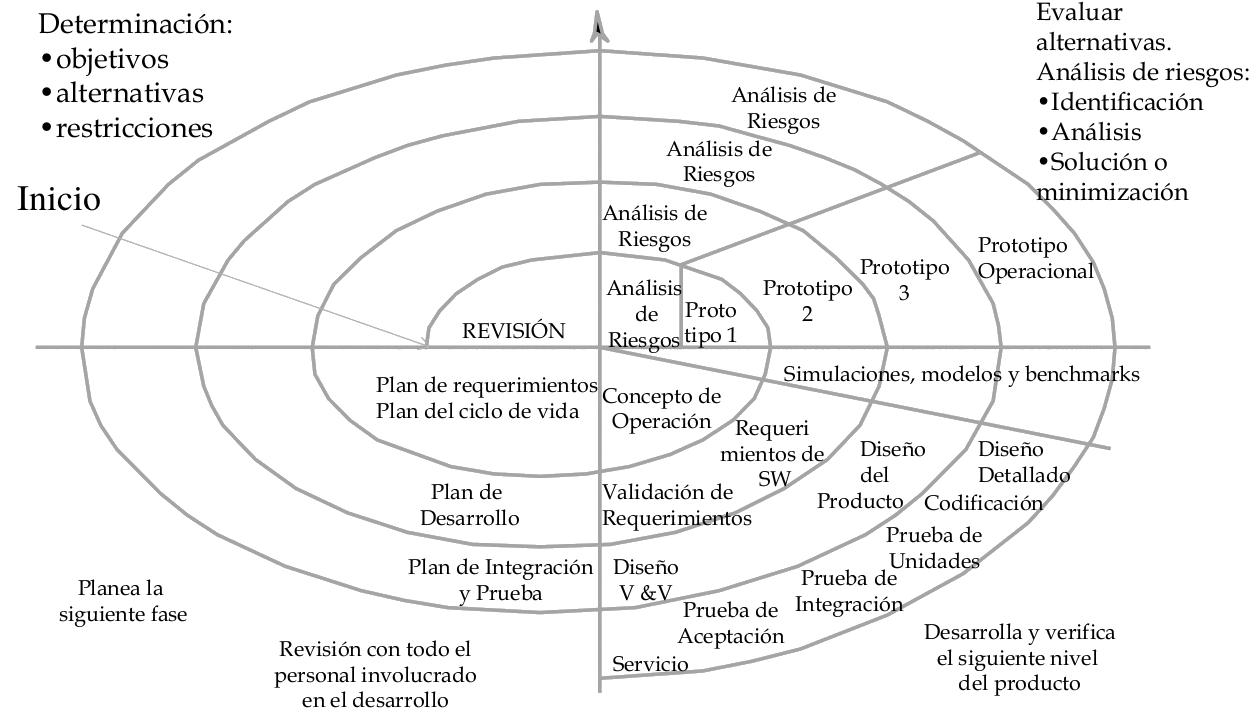
\includegraphics[width=0.9\linewidth]{Resources/Tema3/modeloEspiral.png}
   \caption{Etapas del modelo en espiral.}
   \label{fig:modeloEspiral}
\end{figure}

Es un \textbf{modelo iterativo que combina las principales ventajas del modelo de ciclo de vida en cascada y el modelo de construcción de prototipos}. Su principal característica es incorporar el \textbf{análisis de riesgos} en el propio ciclo de vida, de modo que los prototipos son usados para reducir el riesgo, incluso permitiendo finalizar el proyecto antes de embarcarse en el desarrollo final si no se considera viable.\\

\textbf{Nota:} \textit{Mientras que el modelo iterativo toma la filosofía \uline{iterativa} del desarrollo de prototipos, el modelo en espiral toma directamente las ventajas de realizar prototipos.}


\subsection{Descripción del modelo}

El proceso se representa como una espiral, en donde cada ciclo representa una fase del proceso, en función de lo que mejor se ajuste al proyecto; por ejemplo, el ciclo más interno puede relacionarse con la factibilidad, el siguiente con la definición de requistios, el siguiente, con el diseño, etc. Siempre se actúa en función a los riesgos que el proyecto presente, y por ello se incluyen las actividades de la gestión de riesgos para reducirlos.

Se definen un total de cuatro sectores:

\begin{enumerate}
   \item \textbf{Definición de objetivos}: Objetivos de la fase actual y restricciones con las que deben alcanzarse. Finaliza con la identificación de diferentes alternativas que permitirían alcanzar estos objetivos.
   \item \textbf{Análisis de riesgos}: Se identifican los riesgos de las diferentes alternativas, así como tratarlos, con el objetivo de escoger una de las alternativas.
   \item \textbf{Desarrollo y validación}: Se realiza el análisis de viabilidad de las alternativas y, si se ha reducido el riesgo a niveles aceptables, se realizan las actividades de ingeniería que construyen el producto; es decir, se general entregables de los procesos clásicos, siguiendo, por ejemplo, un ciclo en cascada.
   \item \textbf{Revisión y planificación}: \uline{Todas las personas implicadas}, incluso clientes, revisan los productos desarrolladores y se planificaría la ejecución del siguiente ciclo. Se finaliza con la toma de decisión de finalizar o continuar el proyecto.
\end{enumerate}


\subsection{Ventajas}

\begin{itemize}
   \item Es mucho más realista que el ciclo de vida clásico.
   \item Permite la utilización de prototipos en cualquier etapa de la evolución del proyecto.
   \item Existe un reconocimiento explícito de las alternativas para realizar un proyecto.
   \item Existe una identificación de los riesgos, junto con las diferentes maneras de tratarlos, eliminando las ilusiones de avance.
   \item Se adapta a cualquier tipo de actividad, incluso alejadas de un ciclo de vida tradicional, como la consulta a asesores externos.
\end{itemize}


\subsection{Desventajas}
\begin{itemize}
   \item El modelo en espiral se adapta bien a los desarrollos internos, pero necesita un ajuste para la contración de software, al no contar con la flexibilidad para ajustar el desarrollo etata por etapa (por ejemplo, aplazar decisiones, pararse en miniespirales para realizar secciones críticas con precaución, etc.).
   \item Requiere expertos en la evaluació de riesgos, para realizar evaluaciones apropiadas y no abocarse al desastre.
   \item Resulta difícil de controlar, y de convencer al cliente de que es manejable.
\end{itemize}

\textbf{Nota:} \textit{En todo caso, podría plantearse la realización de un contracto como una iteración del ciclo en espiral}.


\subsection{Análisis de riesgos}

\subsubsection{Definiciones}

\paragraph{Activos} Elementos de un sistema de información que soportan los objetivos de la organización (presentan un cierto valor). Por ejemplo: equipamiento, redes de comunicación, instalaciones, personas, etc.

\paragraph{Amenazas} Qué puede pasarles a los activos, perjudicándolos consecuentemente. Pueden ser de origen natural, del entorno de trabajo, por defectos en el producto, y causados por las personas de forma accidental o deliberada.

\paragraph{Contramedidas} Medidas de protección desplegadas para que las amenazas no causen tanto daño.

\paragraph{Riesgo} Estimación del grado de exposición a que una amenaza se materialice sobre uno o más activos, causando perjuicios a la organización.

\paragraph{Análisis de riesgos} Proceso para estimar la magnitud de los riesgos a los que está expuesta una organización.

\paragraph{Proceso de gestión de riesgos} Proceso destinado a modificar un riesgo, para reducir su impacto.

\begin{figure}[H]
   \centering
   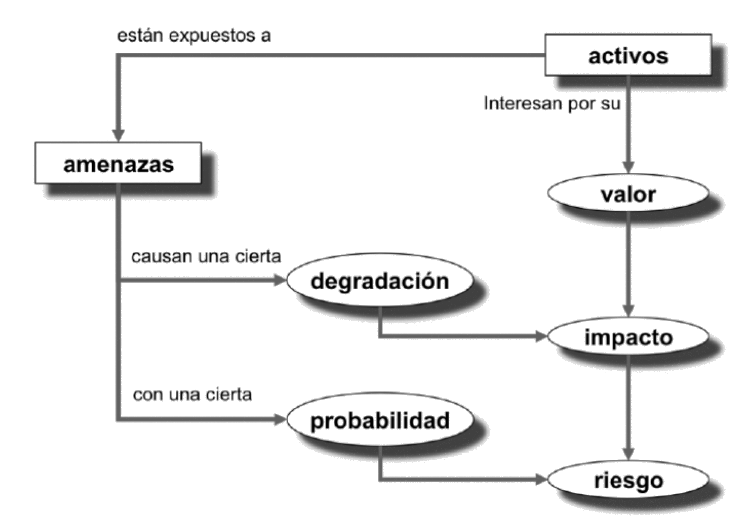
\includegraphics[width=0.6\linewidth]{Resources/Tema3/relacionesDefinicionesRiesgos.png}
   \caption{Elementos del análisis de riesgos potenciales.}
   \label{fig:relacionesDefinicionesRiesgos}
\end{figure}

\subsubsection{Anticipación a los riesgos}

Consta de cuatro actividades principales:

\begin{enumerate}
   \item \textbf{Identificar los riesgos} Se identifican los activos relevantes, a qué amenazas están expuestos, y los riesgos asociados. \textit{Sommerville} clasifica los riesgos en:
      
      \begin{itemize}
         \item Del negocio: Afectan a la organización (riesgos de mercado, mala reputación\ldots).
         \item Del proyecto: Afectan a la calendarización y los recursos.
         \item Del producto: Afectan a la calidad del producto.
      \end{itemize}

   \item \textbf{Análisis de riesgos}: Se evalua, empleando una escala a intervalos y según la experiencia de los expertos, la probabilidad de que cada riesgo ocurra (baja, moderada y alta, por ejemplo), así como sus consecuencias o impacto (catastrófico, grave, tolerable y e insignificante, por ejemplo). A pesar de emplear una escala a intervalos, cada uno de estos debe sustentarse sobre medidas objetivas; por ejemplo, un riesgo tolerable será aquel cuyo impacto no excede los márgenes temporales o económicos del proyecto. Esta actividad concluye con la elaboración de una lista ordenada de riesgos por importancia.

   \item \textbf{Planificación de riesgos}:
         Tras escoger aquellos riesgos más prioritarios, se establecen estrategias para gestionarlos, en base a la experiencia de nuevo:
         \begin{itemize}
            \item Estrategias de prevención.
            \item Estrategias de minimización.
            \item Planes de contingencia: estar preparados para lo peor.
            \item Transferencia: subcontratación de expertos que gestionen y \uline{se responsabilicen} de la gestión del riesgo.
         \end{itemize}
   \item \textbf{Gestión de riesgos}: Supervisar el desarrollo del proyecto continuamente, de forma que se detecten los riesgos tan pronto como aparezcan. Para ello, se definen indicadores cuatificables para cada riesgo, así como sus umbrales de alerta.
\end{enumerate}

\begin{figure}[H]
   \centering
   \includegraphics[width=0.7\linewidth]{Resources/administracionRiesgo.jpg}
   \caption{Administración del riesgos.}
   \label{fig:administracionRiesgo}
\end{figure}





\section{Metodologías ágiles}

Cabe destacar, en todo lo visto hasta el momento, el esfuerzo puesto en:

\begin{itemize}
   \item Documentar los proyectos.
   \item Buscar posibles fallos y seguir las correcciones y modificaciones que suponen, en lugar de centrarse en construir el software en sí.
   \item Garantizar la calidad del producto mediante un seguimiento riguroso de los procesos de construcción.
   \item Modificar los documentos resultantes, dado que no permanecen inmutables en el tiempo.
\end{itemize}

Como se puede ver, estas metodologías pesadas presentan una aproximación sistemática y disciplinada, con procesos fuertemente orientados a la documentación: la documentación no es un objetivo sino el medio para lograrlo y con calidad, y el formalismo da calidad a pesar de ralentizar el desarrollo.
%Sorprendente estos dos párrafos están bien.

El desarrollo ágil defiende la renuncia a utilizar estos modelos perfectos, se basa únicamente en que sean lo \uline{suficientemente buenos}. Tratan de \textbf{centrar los esfuerzos en presentar un incremento software ejecutable}, restando importancia a los productos de trabajo intermedio, que no siempre es bueno.\\

En el manifiesto para el desarrollo ágil, firmado por \textit{Kent Beck} entre otros, se establecía la valoración de:

\begin{itemize}
   \item Individuos e intenciones sobre los procesos.
   \item software en funcionamiento sobre la documentación.
   \item Colaboración con el cliente sobre el contrato.
   \item Respuesta al cambio sobre el seguimiento de un plan.
\end{itemize}

Como se puede ver, estos modelos resultan ser una corriente opuesta a la tradicional, no con el objetivo de eliminarlos, sino de solventar sus limitadas capacidades de adaptación al cambio, dada la fragilidad de los requisitos y la variabilidad del entorno, y la disciplina de trabajo exigida a las personas.\\

\subsection{Variabilidad del entorno}

Las metodologías ligeras proponen una aproximación incremental en donde se valora la entrega frecuente; por ejemplo, desarrollando incrementos tras un par de semanas o de meses. Estos son valorados por el cliente, entrando a ser partícipe del proceso de software, para que ofrezca el \textit{feedback} necesario, como nuevos requisitos o prioridades.

\subsection{Fragilidad por las debilidades humanas}

En contraposición a exigir una gran disciplina al personal para asegurar que los procesos se desarrollan correctamente, las metodologías ligeras aceptan tolerancia en la aplicación de los modelos, permitiendo que estos se adapten al equipo, y no al revés.\\

Algunos de los rasgos con los que las personas deberían contar son: competencia, enfoque común (entregar un incremento a tiempo), colaboración entre todos los \textit{stakeholders}, habilidades y técnicas para la toma de decisiones, capacidad de resolución de problemas ambigüos (debido al cambio), confianza y respeto mutuo, y organización propia para lograr los objetivos.

\subsection{Diferentes modelos de proceso}

\begin{itemize}
   \item Programación Extrema (PE).
   \item Desarrollo Adaptativo del Software (DAS).
   \item SCRUM.
   \item Cristal.
   \item Desarrollo conducido por características (DCC).
   \item Modelado Ágil.
\end{itemize}

\subsection{Modelado ágil}

A \textbf{alto nivel}, es una \textbf{colección de valores, pricipios y prácticas} (en resumen, buenas prácticas) que poder aplicar para realizar modelado y documentación de forma efectiva y ligera en un proyecto de desarrollo de software. Por ejemplo, es habitual la práctica de \textit{Test-Driven Development}, que consta a su vez de las dos prácticas de \textit{Test-First Development} y de refactorización.\\

Al final, el modelado ágil puede ser tomado más como una filosofía que como una metodología:

\begin{itemize}
   \item Modelar con un propósito: Trabajar siempre con un objetivo en mente.
   \item Conocer los modelos y notaciones disponibles, y usar el más apropiado para cada situación.
   \item Viajar ligero: Conservar sólo la documentación o modelos que proporcionarán valor a largo plazo, y que deberán recibir por lo tanto un mantenimiento.
   \item El contenido es más importante que la representación: Solo es necesario que un modelo pueda ser interpretado por la audiencia a la que está dirigido.
   \item Adaptar a las necesidades del equpo.
\end{itemize}

\subsection{Programación extrema}

\begin{figure}[H]
   \centering
   \includegraphics[width=0.7\linewidth]{Resources/programacionExtrema.jpg}
   \caption{Etapas de la programación extrema.}
   \label{fig:programacionExtrema}
\end{figure}

Utiliza, preferiblemente, un enfoque orientado a objetos, y abarca un conjunto de reglas y prácticas que ocurren las siguientes cuatro actiividades:

\begin{enumerate}

   \item \textbf{Planificación}:
         
      \begin{itemize}
            \item \textbf{Creación de historias de usuario}: Describen características y funcionalidades requeridas (permiten establecer requisitos); cada historia se asemeja a un caos de uso, es escrita por el cliente, y este le asigna una prioridad.
            \item \textbf{Estimación del tiempo de implementación}: Los miembros del equipo evalúan cada historia y asignan un coste en semanas de desrollo; si es superior a tres semanas, se segmenta la historia.\\
            \textbf{Nota:} \textit{Pueden escribirse historias en cualquier momento.}
            \item \textbf{Plan de construcción}: Los clientes y el equipo se reúnen para decidir qué historias hay en el siguiente incremento del software, priorizando siguiendo una de las siguientes vías:
                  \begin{itemize}
                     \item Todas las historias serán implementadas de un modo inmediato.
                     \item Las historias con \textbf{valor más alto} se implementarán al \textbf{principio}.
                     \item Las historias de \textbf{mayor riesgo} se implementarán al \textbf{principio}.
                  \end{itemize}
            \item \textbf{Cálculo de la velocidad del proyecto}: Tras cada lanzamiento, se recoge el número de historias implementadas, con la intención de:
                  \begin{itemize}
                     \item Ayudar a estimar futuras fechas de entrega y programaciones.
                     \item Determinar si, hasta el momento, ya se ha realizado algún compromiso no viable.
                  \end{itemize}
         \end{itemize}


   \item \textbf{Diseño}: Sigue el principio KISS (\textit{Keep It Simple, Stupid}), de modo que solo se implementa lo requerido, y se apoya en:
         % https://en.wikipedia.org/wiki/KISS_principle El stupid es importante. Porque somos estúpidos y debemos recordarlo.
         \begin{itemize} %Mejor así.
            \item \textbf{Tarjetas CRC} (Colaborador--Responsabilidad--Clase).
            \item \textbf{Soluciones de Pico}: Si se presenta un problema difícil, se recomienda construir un prototipo para probar dicha parte y analizarlo, de modo que se reduzca el riesgo a la hora de comenzar la verdadera implementación.
            \item \textbf{Refabricación} (\textit{Refactoring}): Cambiar un sistema de software de tal manera que no altere el comportamiento externo del código y que mejore la estructura interna (mejorar el diseño del código después de que haya sido escrito).
            \item \textbf{Diseño como artefacto}: Se permite la modificación del diseño durante todas las fases de la construcción.
         \end{itemize}

   \item \textbf{Codificación}:
   
   \begin{itemize}
      \item Después de realizar el trabajo de diseño preliminar, se prefiere crear las \textbf{pruebas de unidad que ejerciten cada una de las historias, antes que el código} de las clases. Así, el desarrollador se centra en implementar lo necesario para pasar la prueba de unidad y, una vez escrito el código, puede evaluarse de inmediato.
      \item Un concepto clave durante la codificación es la programación en pareja, con el objetivo de mejorar la capacidad de resolución de problemas y asegurar la calidad. En la práctica, cada persona tiene un papel sutilmente diferente.
      \item Una vez unos desarrolladores finalizan su trabajo, el código escrito debe integrarse con el trabajo de otros; mediante esta estrategia de integración continua, se evitan mayores problemas de compatibilidad e interfaz. Se realizan ``pruebas de humo'', que son pruebas de integración poco exhaustivas de todo el sistema con las que detectar los errores más importantes.
   \end{itemize}

   \item \textbf{Pruebas}:
         \begin{itemize}
            \item \textbf{Pruebas diarias}: Comprenderían, principalmente, las pruebas de unidad e integración, y deberían organizarse de forma que puedan ser automatizadas. Así, si se realizan a diario, se proporciona al equipo un indicador de progreso, así como una alarma fiable en caso de que las cosas vayan mal.
            \item \textbf{De aceptación o del cliente}: Estando especificadas por el cliente, se enfocan en las características generales y la funcionalidad del sistema, siempre sobre aspectos que el cliente pueda revisar. Se derivan de las historias de usuario implementadas.
         \end{itemize}
\end{enumerate}
